\documentclass[UTF8]{ctexart}

\usepackage{titlesec}
\titleformat{\section}[hang]{\normalfont\Large\bfseries}{\thesection}{1em}{}[]
\titlespacing{\section}{10pt}{\baselineskip}{10pt}
\usepackage{geometry}
\usepackage{listings}
\usepackage{xcolor}
\usepackage{graphicx}
\usepackage{fancyhdr}
\pagestyle{fancy}
\fancyhead{} % 清空页眉内容
\lstset{
    basicstyle=\ttfamily,
    columns=fullflexible,
    breaklines=true,
    frame=single,
    backgroundcolor=\color{lightgray!20},
    numbers=left,
    numberstyle=\small,
    numbersep=8pt,
    keywordstyle=\color{blue},
    commentstyle=\color{green!60!black},
    stringstyle=\color{red},
    showstringspaces=false,
    tabsize=4,
    escapeinside=`'
}

\title{利用SVD和PCA算法进行图像压缩}
\author{姓名:李哲远~~~~~~~~~学号:202352110331}
\date{\today}

\begin{document}
\maketitle

\section{SVD奇异值分解算法}
奇异值分解(Singular Value Decomposition,简称SVD)是一种常用的矩阵分解方法,用于将一个矩阵分解为三个矩阵的乘积。SVD在许多领域中都有广泛的应用,如数据降维、图像压缩、推荐系统等。

\subsection{数学公式表示}
SVD的数学公式表示如下:
给定一个$m \times n$的矩阵$A$,其SVD表示为:

\[
A = U \Sigma V^T
\]

其中,$U$是一个$m \times m$的酉矩阵,表示$AA^T$的特征向量构成的矩阵;$\Sigma$是一个$m \times n$的对角矩阵,表示$A$的奇异值构成的矩阵;$V$是一个$n \times n$的酉矩阵,表示$A^TA$的特征向量构成的矩阵。

\subsubsection{几何意义}


$U$是一个正交矩阵,表示旋转操作;$\Sigma$是一个对角矩阵,表示缩放操作;$V$是另一个正交矩阵,表示再旋转操作。

具体而言,SVD的几何意义可以解释如下:

$U$表示将原始空间中的向量旋转到一个新的坐标系中。这个新坐标系的基向量是$U$的列向量,它们是原始坐标系中的标准正交基向量的旋转版本。

$\Sigma$表示在每个坐标轴上的缩放因子。$\Sigma$的对角线上的元素称为奇异值,它们表示原始向量在每个旋转后的坐标轴上的缩放程度。奇异值按照降序排列,因此,前面的奇异值对应着更重要的特征。

$V$表示将旋转后的向量再次旋转回原始坐标系。$V$的列向量是原始坐标系中的标准正交基向量的再旋转版本。

总的来说是将一个矩阵通过旋转,拉伸,再旋转,而拉伸即用中间的奇异值矩阵进行表示。通过SVD,我们可以将一个矩阵 $A$ 表示为一系列几何操作的组合,从而揭示了原始数据的主要几何特征。SVD在降维、信号处理、图像压缩等领域中具有广泛的应用,可以提取数据的重要特征、去除噪声和冗余信息,并帮助理解数据的结构和模式。

\subsubsection{SVD算法步骤}
SVD算法的基本步骤如下:


\begin{enumerate}
  \item 给定一个$m \times n$的矩阵$A$,其中$m$是行数,$n$是列数。
  \item 计算$A$的转置矩阵$A^T$与$A$的乘积$AA^T$。
  \item 对$AA^T$进行特征值分解,得到特征值和特征向量。
  \item 计算$A^T$的转置矩阵$(A^T)^T$与$A^T$的乘积$A^TA$。
  \item 对$A^TA$进行特征值分解,得到特征值和特征向量。
  \item 根据特征值和特征向量构建奇异值矩阵$\Sigma$。
  \item 对$A$进行奇异值分解,得到矩阵$U$、$\Sigma$和$V$。
\end{enumerate}


\subsection{图像压缩算法实现}
这里主要使用python实现对目标图片进行压缩。通过查阅相关资料了解到可以通过使用pytorch中的svd函数进行实现,
也可以通过使用python中numpy库中线性代数相关的函数进行分解,这里选择采用第二种方式。其次这次试验要求
处理的图像为一张图像,因此转化为张量形式之后三维的,通道深度为3,分别表示红绿蓝三色。而传统的SVD分解算法
则只能处理二维矩阵形式,也就是灰度图。因此考虑到两种方法对其进行分解,一种是将3维张量reshape成2维,
在进行相关压缩之后再reshape回来。第二种方法是对3个通道分别进行SVD分解,然后再把三个通道叠加成三维张量
的形式。

\subsubsection{方法一}
方法一将3维张量reshape成2维,在进行相关压缩之后再reshape回来,并使用pytorch中的SVD函数进行处理。
代码如下:
\begin{lstlisting}[language=Python]
  import numpy as np
  import matplotlib.pyplot as plt
  import torch
  # `读取图片'
  imag = plt.imread('butterfly.bmp')
  
  tensor_image = torch.tensor(imag)
  reshaped_image = tensor_image.reshape(-1,437)
  float_image = reshaped_image.float()
  U, S, V = torch.svd(float_image)
  
  # `误差'
  errors=[]
  
  # `按照奇异值数量倒序进行图片展示,每次减少25个奇异值'
  for k in range(len(S), 0, -25):
      # `分解'
      
      compressed_S = np.diag(S[:k])
      compressed_U = U[:, :k]
      compressed_V= V[:k, :]
  
  
      # `计算'
      reconstructed_array = np.dot(compressed_U, np.dot(compressed_S, compressed_V))
      
  
      # `回滚'
      reconstructed_image_array = reconstructed_array.reshape(imag.shape)
      reconstructed_image = reconstructed_image_array.astype(np.uint8)
      
      # `误差分析'
      diff = imag - reconstructed_image
      mse = np.mean(np.square(diff))
      errors.append(mse)
      
      # # `图片展示,如需要可以将注释打开'
      # plt.imshow(reconstructed_image)
      # plt.show()
  
  # `误差分析'
  plt.plot(range(len(S), 0, -25),errors)
  plt.xlabel('`奇异值数'',fontproperties='SimHei')
  plt.ylabel('`均方误差'',fontproperties='SimHei')
  plt.show()
  
  \end{lstlisting}
  下面分别为误差图和压缩后图像:

  \begin{figure}[htbp]
    \centering
    \begin{minipage}{0.4\textwidth}
      \centering
      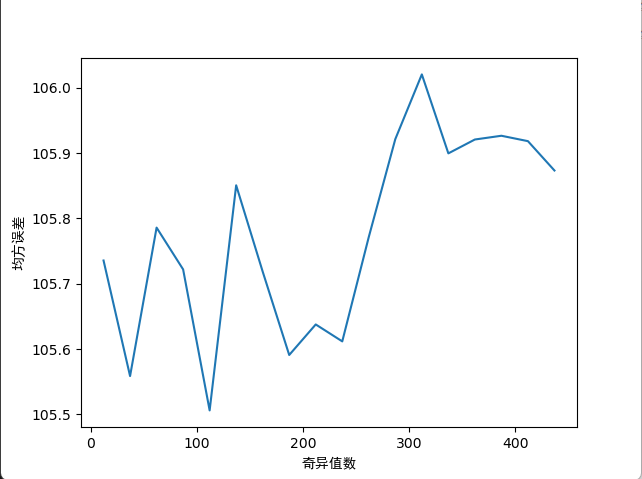
\includegraphics[width=\textwidth]{1.png}
      \caption{法一误差图}
      \label{fig:subfig1}
    \end{minipage}
    \hspace{1cm} % 调整两张图片之间的水平间距
    \begin{minipage}{0.4\textwidth}
      \centering
      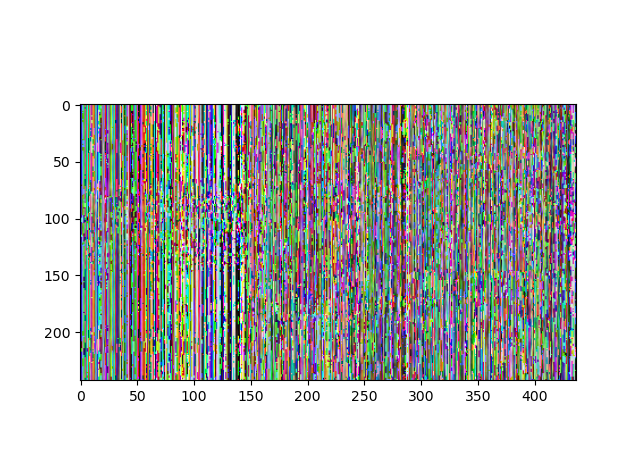
\includegraphics[width=\textwidth]{2.png}
      \caption{第一次压缩图像}
      \label{fig:subfig2}
    \end{minipage}
  
    \label{fig:combined}
    \end{figure}
可以看到如果先将三维张量压缩为二维在进行SVD分解,之后再还原成三维的方法是不行的。造成这种结果的原因
可能是在将三个通道压缩成一个通道之后,奇异值所代表的特征是三个通道叠加的,在进行相关压缩之后再reshape回来后
就会出现一些错误。
\subsubsection{方法二}
第二种方法是对3个通道分别进行SVD分解,采用的是numpy库中关于线性代数的相关函数。把三个通道拆分为R,G,B,对三个
不同的矩阵分别处理,之后再叠加,代码如下:
\begin{lstlisting}[language=Python]
  import numpy as np
  import matplotlib.pyplot as plt
  
  # `读取图片'
  imag = plt.imread('butterfly.bmp')
  
  # `图片深度是3,拆分为深度1的3个矩阵分别进行分解'
  red_channel = imag[:, :, 0]
  green_channel = imag[:, :, 1]
  blue_channel = imag[:, :, 2]
  
  # `进行分解'
  U_red, S_red, V_red = np.linalg.svd(red_channel)
  U_green, S_green, V_green = np.linalg.svd(green_channel)
  U_blue, S_blue, V_blue = np.linalg.svd(blue_channel)
  
  # `误差'
  errors=[]
  
  # `按照奇异值数量倒序进行图片展示,每次减少25个奇异值'
  for k in range(len(U_red), 0, -25):
      # `分解三个深度'
      compressed_S_red = np.diag(S_red[:k])
      compressed_S_green = np.diag(S_green[:k])
      compressed_S_blue = np.diag(S_blue[:k])
      # `UV分解'
      compressed_U_red = U_red[:, :k]
      compressed_V_red = V_red[:k, :]
      compressed_U_green = U_green[:, :k]
      compressed_V_green = V_green[:k, :]
      compressed_U_blue = U_blue[:, :k]
      compressed_V_blue = V_blue[:k, :]
      # `计算'
      compressed_red_channel = np.dot(compressed_U_red, np.dot(compressed_S_red, compressed_V_red))
      compressed_green_channel = np.dot(compressed_U_green, np.dot(compressed_S_green, compressed_V_green))
      compressed_blue_channel = np.dot(compressed_U_blue, np.dot(compressed_S_blue, compressed_V_blue))
      # `合并三个深度'
      compressed_imag = np.stack([compressed_red_channel, compressed_green_channel, compressed_blue_channel], axis=2)
      compressed_imag = compressed_imag.astype(np.uint8)
      # `误差分析'
      diff = imag - compressed_imag
      mse = np.mean(np.square(diff))
      errors.append(mse)
      # # `图片展示,如需要可以将注释打开'
      # plt.imshow(compressed_imag)
      # plt.show()
  # `误差分析'
  plt.plot(range(len(U_red), 0, -25),errors)
  plt.xlabel('`奇异值数'',fontproperties='SimHei')
  plt.ylabel('`均方误差'',fontproperties='SimHei')
  plt.show() 
 \end{lstlisting}
 下面为误差图:
 
 \begin{figure}[htbp]
  \centering
  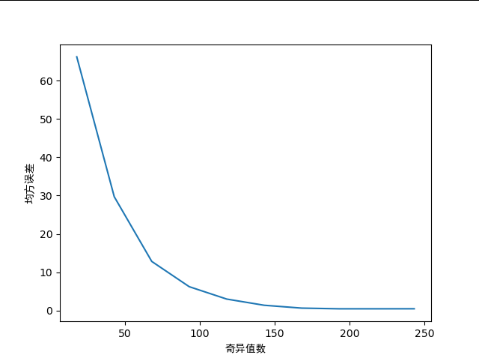
\includegraphics[width=0.5\textwidth]{3.png}
  \caption{SVD分解误差}
  \label{fig:example}
\end{figure}

该误差图是将奇异值从大到小进行排序后,依次减少25个奇异值并分析其误差画出来的折线图,可以看出在初期
减少奇异值的时候误差变化并不大,原因在于刚开始减小的是一些数值比较小的奇异值,可以解释为这些奇异值
对该图像的特征并没什么影响。 

下面展示压缩后的图片:

\begin{figure}[htbp]
  \centering
  \begin{minipage}{0.4\textwidth}
    \centering
    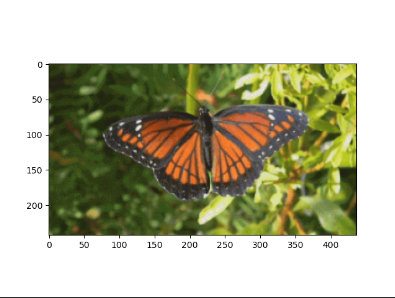
\includegraphics[width=\textwidth]{4.png}
    \caption{第八张图(去除200个奇异值)}
    \label{fig:subfig1}
  \end{minipage}
  \hspace{1cm} % 调整两张图片之间的水平间距
  \begin{minipage}{0.4\textwidth}
    \centering
    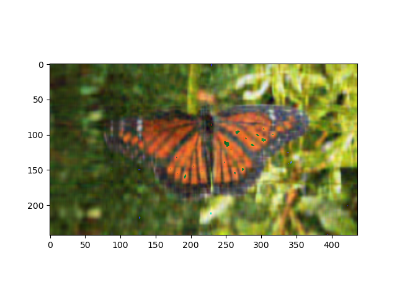
\includegraphics[width=\textwidth]{10.png}
    \caption{第十张图(去除250个奇异值)}
    \label{fig:subfig2}
  \end{minipage}

  \label{fig:combined}
  \end{figure}

  
  可以发现在去除200个奇异值后,图片跟原图片的差距还是很小,再去除50个之后就造成了较大的误差。
  这就是因为前几个比较大的奇异值对图像的影响比较大,因此可以去除后面比较小的奇异值来实现图像压缩。
\section{PCA主成分分析法}
主成分分析(Principal Component Analysis,简称PCA)是一种常用的数据降维和特征提取技术。它通过线性变换将原始数据投影到一个新的坐标系中,使得投影后的数据具有最大的方差。在图片压缩中,PCA可以用于降低图像的维度,从而实现图片的压缩。
\subsection{数学公式表示}
给定一个$m \times n$的矩阵$D$,其PCA表示为:

\[
D=S^{-1}R^{-1}D'~~~~~~~~~~~~D'= RSD
\]

其中,$D'$是待分析的矩阵,$R$表示对该矩阵进行旋转操作,主要目的是找到数值方差最大的作为主轴,$D$是一个对角矩阵
目的是为了对图片进行拉伸操作,$D$则为处理过后的矩阵。
\subsection{几何意义}
给定一个包含$n$个样本的数据集$\mathbf{X}={\mathbf{x}_1, \mathbf{x}_2, \ldots, \mathbf{x}_n}$,其中每个样本$\mathbf{x}_i$是一个$d$维向量。PCA算法的目标是找到一个$d$维的正交变换矩阵$\mathbf{W}$,将原始数据$\mathbf{X}$投影到新的坐标系中,使得投影后的数据具有最大的方差。
\subsection{图像压缩算法实现}
\textbf{1. 数据预处理:} 首先,将图片转换为灰度图像。如果图片是彩色图像,可以将其转换为灰度图像,这样每个像素只有一个灰度值。然后,将每个像素的灰度值归一化到0到1的范围,以便统一数据的尺度。

\textbf{2. 构建数据矩阵:} 将归一化后的图片数据转换为一个数据矩阵,其中每一列代表一个样本,每一行代表一个特征(像素)。

\textbf{3. 计算协方差矩阵:} 对数据矩阵进行协方差计算,得到一个协方差矩阵。协方差矩阵描述了不同特征之间的相关性。

\textbf{4. 特征值分解:} 对协方差矩阵进行特征值分解,得到特征值和对应的特征向量。特征向量代表了原始数据在新坐标系中的投影方向,而特征值表示数据在对应特征向量方向上的方差。

\textbf{5. 选择主成分:} 根据特征值的大小,选择最大的几个特征值对应的特征向量作为主成分。主成分对应的特征向量表示了数据中最重要的方向。

\textbf{6. 降维:} 将原始数据矩阵与选取的主成分特征向量相乘,得到降维后的数据矩阵。降维后的数据矩阵将保留了最重要的特征,同时减少了数据的维度。

\textbf{7. 重构:} 将降维后的数据矩阵与选取的主成分特征向量的转置相乘,得到重构后的数据矩阵。重构后的数据矩阵可以近似地还原原始数据。

\textbf{8. 逆归一化:} 将重构后的数据矩阵进行逆归一化,将像素值恢复到原始范围。

通过选择合适的主成分数量,可以在保留较高图像质量的同时实现图像的压缩。通常,选择的主成分数量越少,压缩比例越高,但图像质量也会相应降低。

需要注意的是,PCA压缩是有损压缩,因为压缩后的图像无法完全恢复为原始图像。压缩比例和图像质量之间存在着权衡。

具体代码如下:
\begin{lstlisting}[language=Python]
  import numpy as np
import matplotlib.pyplot as plt
from sklearn.decomposition import PCA
from PIL import Image

# `读取图片'
imag = plt.imread('butterfly.bmp')

image_array = np.array(imag)
# `将图像重塑为二维矩阵'
reshaped_array = imag.reshape(-1, 437)

# `误差'
errors=[]

for n_components in range(437, 0, -25):
    # `创建PCA对象,指定要保留的主成分数量'
    pca = PCA(n_components=n_components)

    # `执行PCA降维'
    compressed_array = pca.fit_transform(reshaped_array)

    # `重构压缩后的数据'
    reconstructed_array = pca.inverse_transform(compressed_array)

    # `将数据形状转换回图像尺寸'
    reconstructed_image_array = reconstructed_array.reshape(imag.shape)


    # `将重构的数据转换回图像'
    reconstructed_image = reconstructed_image_array.astype(np.uint8)

    reconstruction_error = np.mean(np.square(reconstructed_image - image_array))
    errors.append(reconstruction_error)

    # `图片展示,需要则打开'
    # plt.imshow(reconstructed_image)
    # plt.show()

plt.plot(range(437, 0, -25),errors)
plt.xlabel('`保存的维数'',fontproperties='SimHei')
plt.ylabel('`均方误差'',fontproperties='SimHei')
plt.show()
  
\end{lstlisting}
得到的均方误差关于保存的维数折线关系图:
\begin{figure}[htbp]
  \centering
  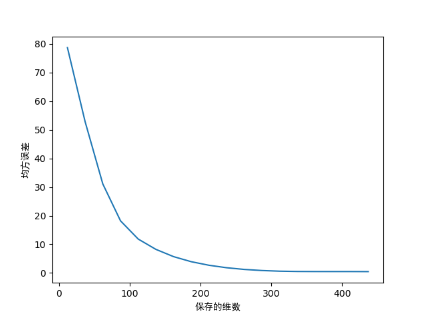
\includegraphics[width=0.5\textwidth]{5.png}
  \caption{PCA主成分分析法误差}
  \label{fig:example}
\end{figure}

同时展示压缩后的图片:

\begin{figure}[htbp]
  \centering
  \begin{minipage}{0.4\textwidth}
    \centering
    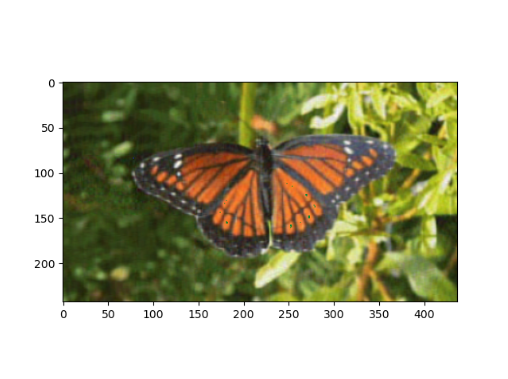
\includegraphics[width=\textwidth]{6.png}
    \caption{第八张图(去除200个成分)}
    \label{fig:subfig1}
  \end{minipage}
  \hspace{1cm} % 调整两张图片之间的水平间距
  \begin{minipage}{0.4\textwidth}
    \centering
    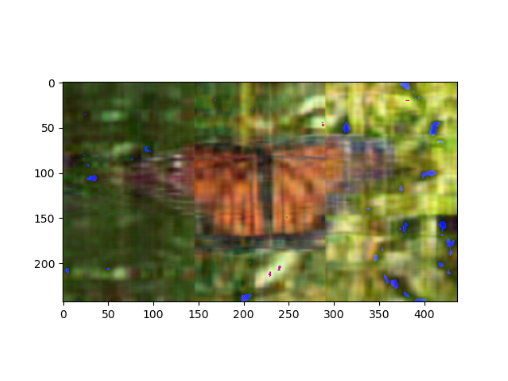
\includegraphics[width=\textwidth]{9.png}
    \caption{第十张图(去除250个成分)}
    \label{fig:subfig2}
  \end{minipage}

  \label{fig:combined}
  \end{figure}

\section{总结}
从图像压缩上对比两种算法,SVD只能处理灰度图,如果想要处理彩色图片,可能需要对三个通道分别处理。
而PCA主成分分析法则可以直接通过将三维张量reshape成二维矩阵的方式进行压缩,最后再转化为三维张量
(可能不同通道之间在算法进行时没有进行相互的影响?)。
而误差上较为类似,均是在去除大量低奇异值的或成分时候造成较小的误差。

而从数学上来讲,PCA 是一种基于协方差矩阵的线性降维方法,SVD 是一种矩阵分解方法。而且SVD中的右奇异值矩阵V
就是PCA主成分的方向,所以当数据量很大的时候可以通过求SVD分解得到有奇异值矩阵V作为PCA的主成分,
这样就避免了求协方差矩阵。


\end{document}